
%------------------------------------------------

\section{Properties of probability}\index{probability!property}
\label{sec:prop_of_prob}

\subsection{Bayes' theorem for discrete events}\index{Bayes' theorem}
\label{subsec:bayes__discrete}

Recall the law of conditional probability (with two sets $A$ and $B$)

\begin{equation}
	P(A \wedge B) = P(B \mid A) P(A) = P(A \mid B) P(B)
\end{equation}

therefore:

\begin{equation}\label{eq:bayes__discrete}
	P(A \mid B) = \frac{P(B \mid A) P(A)}{P(B)}
\end{equation}

More generally, if $A_{i} = A_{1}, \cdots, A_{n}$ are \mono{exclusive and exhaustive} sets, and if $B$ is any event:
\begin{equation}\label{eq:bayes__discrete_general}
	P(A_{i} \mid B)
	= \frac{P(B \mid A_{i}) P(A_{i})}
		{\sum_{i}{P(B \mid A_{i}) P(A_{i})}}
\end{equation}

\begin{itemize}
	\item $P(A_{i})$ is the “prior probability”\index{prior probability} of $A_{i}$, i.e. the probability of set $A_{i}$ before the knowledge that event $B$ has occurred.
	\item $P(A_{i} \mid B)$ is the “posterior probability”\index{posterior probability} of $A_{i}$, i.e. the probability of set $A_{i}$ after having collected the information that event $B$ has occurred.
\end{itemize}

\newthought{Example}: measuring protons with particle detectors (Figure~\ref{fig:Bayes__theorem_proton}):

\begin{itemize}
	\item $P(B) = P(+ \wedge p) + P(+ \wedge n) = $ probability of any particle giving a triggered event.
	\item $P(A) = P(+ \wedge p) + P(0 \wedge p) = $ probability of a proton hitting the detector.
	\item $P(B \mid A) = \frac{P(+ \wedge p)}{P(+ \wedge p) + P(0 \wedge p)} = $ probability of a proton giving a triggered event.
	\item $P(A \mid B) = \frac{P(+ \wedge p)}{P(+ \wedge p) + P(+ \wedge n)} = $ probability of a triggered event to be induced by a proton.
\end{itemize}

\begin{figure}
	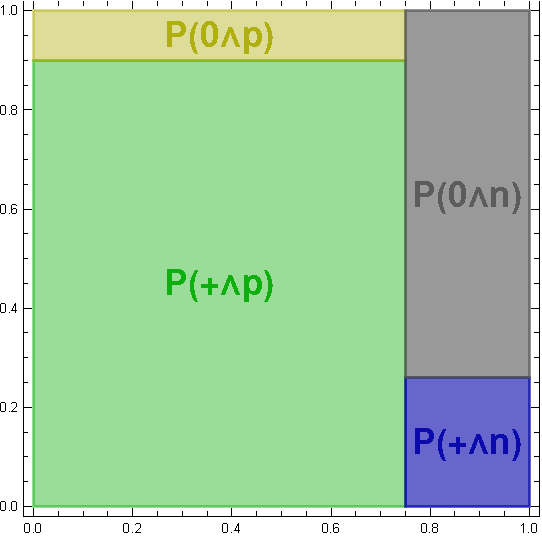
\includegraphics{probability/Bayes__theorem.pdf}
	\caption[Venn diagram of Bayes' theorem.][6pt]{Venn diagram of Bayes' theorem.}
	\label{fig:Bayes__theorem_proton}
\end{figure}

\subsection{Bayes' theorem for hypotheses testing and parameter estimation}\index{hypothesis test}
\label{subsec:bayes__hypo}

\newthought{Assume} $H_{0}$, $H_{1}$ are a complete set of hypotheses, i.e. a complete set os physics models describing a given physical phenomenon. 

For example:

\begin{itemize}
	\item $H_{0} = $ background-only hypothesis\index{hypothesis!background-only} = The known physics processors are enough to explain the data.
	\item $H_{1} = $ signal + background hypothesis\index{hypothesis!signal + background} = There is an additional component due to new physics and that we know how to model.
\end{itemize}

$H_{0}$ and $H_{1}$ will depend on some parameters, which can differ between the two hypotheses, but that we will indicate generally as $\vec{\theta} \in \Omega $.

Let's indicate the data with $\vec{x}$.

\paragraph{Parameter estimation}\index{parameter estimation}

\begin{equation}\label{eq:para_esti}
	P( \vec{\theta} \mid \vec{x} )
	= \frac{P( \vec{x} \mid \vec{\theta} ) \pi(\vec{\theta})}
		{\int_{\Omega} {P( \vec{x} \mid \vec{\theta} ) \pi(\vec{\theta})} \,\mathrm{d}\vec{\theta}}
	= \frac{P( \vec{x} \mid \vec{\theta} ) \pi(\vec{\theta})}
		{P( \vec{x})}
\end{equation}

\begin{itemize}
	\item $P( \vec{\theta} \mid \vec{x} ) = $ posterior probability\index{posterior probability} for parameters $\vec{\theta}$ gives the data $\vec{x}$ and the model $H_{0}$ or $H_{1}$. 
		\marginnote{This is valid both for $H_{0}$ and $H_{1}$.}
	\item $P( \vec{x} \mid \vec{\theta} ) = $ probability of obtaining exactly the data $\vec{x}$ gives each possible values of the parameters $\vec{\theta}$.
	\item $\pi(\vec{\theta}) = $ prior probability\index{prior probability} of parameter $\vec{\theta}$ under the assumption of $H_{0}$ or $H_{1}$.
	\item $P(\vec{x}) = $ probability of getting data $\vec{x}$ given any possible value of $\vec{\theta}$ assuming model $H_{0}$ or $H_{1}$.
		\marginnote{In the end, it is a normalization factor.}
\end{itemize}

\newthought{Considering both hypotheses} $H_{0}$ and $H_{1}$:

\begin{equation} 
	P( \vec{\theta}, H_{0} \mid \vec{x} )
	= \frac{P( \vec{x} \mid H_{0}(\vec{\theta}) ) \pi( \vec{\theta}, H_{0} )}
		{\sum_{i}{\int_{\Omega} {P( \vec{x} \mid \vec{\theta}_{i}, H_{i} ) \pi( \vec{\theta}_{i}, H_{i} ) \pi(H_{i})} \,\mathrm{d}\vec{\theta}}}
\end{equation} \marginnote[-6pt]{denominator $\to$ \mono{constant}}

\paragraph{Hypothesis testing}\index{hypothesis test}
\begin{equation}\label{eq:hypo_test}
	P(H_{i} \mid \vec{x})
	= \frac{P(\vec{x} \mid H_{i}) \pi(H_{i})}
		{\sum_{i}{P(\vec{x} \mid H_{i}) \pi(H_{i})}}
\end{equation}

\begin{itemize}
	\item $P(H_{i} \mid \vec{x}) = $ posterior probability\index{posterior probability} for hypothesis $H_{i}$ after measuring the data.
	\item $\pi(H_{i}) = $ prior probability\index{prior probability} for hypothesis $H_{i}$.
		\marginnote{This is the \mono{subjective} part of the method.}
	\item $P(\vec{x} \mid H_{i}) = \int_{\Omega} {P( \vec{x} \mid \vec{\theta}, H_{i} ) \pi(\vec{\theta})} \,\mathrm{d}\vec{\theta} = $ probability of obtaining data $\vec{x}$ gives each possible values of the parameters $\vec{\theta}$ assuming model $H_{i}$.
	\item $\sum_{i}{P(\vec{x} \mid H_{i}) \pi(H_{i})} = $ normalization factor.
\end{itemize}

\newthought{Example}: religious belief.
